\begin{atiTask}[
	title = Orthogonaltrajektorien und Richtungsfeld,
	language = Deutsch
]
	Betrachten Sie die Schar von Hyperbeln, die durch die folgende Gleichung beschrieben wird.
	Dabei stellt $c$ einen reellen Parameter dar.
	\[
		x^2 - 2y^2 = c^2
	\]
	\begin{atiSubtasks}
		\item{\locallabel{a}
			Stellen Sie eine Differentialgleichung auf, die diese Kurvenschar beschreibt.
		}
		\item{\locallabel{b}
			Leiten Sie daraus die Differentialgleichung für die zugehörigen Orthogonaltrajektorien her und skizzieren Sie deren Richtungsfeld.
		}
		\item{\locallabel{c}
			Lösen Sie die Differentialgleichung für die Orthogonaltrajektorien durch die Methode der Trennung der Variablen. Ergänzen Sie Ihre Skizze durch Hyperbeln und Orthogonaltrajektorien für den folgenden Anfangswert.
			\[
				x_0\define 6\separate y_0\define y(x_0)\define 4
			\]
		}
	\end{atiSubtasks}
\end{atiTask}
\begin{atiSolution}
	\begin{atiSubtaskSolutions}
		\item[\localref{a}]{
			Wir nehmen an, dass es sich bei $y$ um eine Funktion auf einer offenen Teilmenge $M\subset\setReal$ handelt und dass der Graph von $y$ die gegebene Gleichung für alle $x\in M$ erfüllt.
			% In diesem Falle lässt sich die gegebene Gleichung für ein $x$ dieser offenen Teilmenge in der folgenden Form schreiben.
			\[
				x^2 - 2y^2(x) = c^2 \implies \leibnizDerivativeOperatorValue{\tilde{x}}{\tilde{x}^2 - 2y^2(\tilde{x})}{x} = \leibnizDerivativeOperatorValue{\tilde{x}}{c^2}{x} \implies 2x - 4y(x)y'(x) = 0
			\]
			Man erhält damit eine Differentialgleichung der folgenden Formen.
			\[
				2yy'=x \separate y'=\frac{x}{2y}\atiPoints[1]
			\]
		}
		\item[\localref{b}]{
			Die Orthogonaltrajektorien müssen demzufolge der folgenden Differentialgleichung genügen.
			Das Richtungsfeld dieser Differentialgleichung wird in der nachfolgenden Skizze abgebildet.
			\[
				y' = -\frac{2y}{x}\atiPoints[1]
			\]
		}
		\item[\localref{c}]{
			Durch Umstellung erhält man eine separierte Differentialgleichung, die sich für die Anfangswerte $x_0\in\setReal\setminus\set{0}{}$ und $y_0\define y(0)\in\setReal\setminus\set{0}{}$ direkt lösen lässt.
			\[
				\frac{y'(x)}{y(x)} = -\frac{2}{x} \implies \integral{x_0}{x}{\frac{y'(s)}{y(s)}}{s} = -2 \integral{x_0}{x}{\frac{1}{s}}{s}
			\]
			\[
				\implies \integral{y_0}{y(x)}{\frac{1}{s}}{s} = \ln\absolute{\frac{y(x)}{y_0}} = \ln\roundBrackets{\frac{y(x)}{y_0}} = -2 \ln\absolute{\frac{x}{x_0}} = -2 \ln\roundBrackets{\frac{x}{x_0}}
			\]
			\[
				\implies y(x) = \frac{y_0x_0^2}{x^2}\atiPoints[1]
			\]
			Setzt man nun $x_0 = 6$ und $y_0 = 4$, so erhält man die folgenden Aussagen.
			\[
				c^2 = x_0^2 - 2y_0^2 = 4 \implies c = \pm 2 \separate y_0x^2_0 = 144 \atiPoints[1]
			\]
			Auch hier sind die entsprechende Hyperbel und die, der Differentialgleichung entsprechenden, Orthogonaltrajektorie in der nachfolgenden Skizze eingezeichnet.
		}
		\begin{figure}[H]
			\center
			\atiPoints[3]
			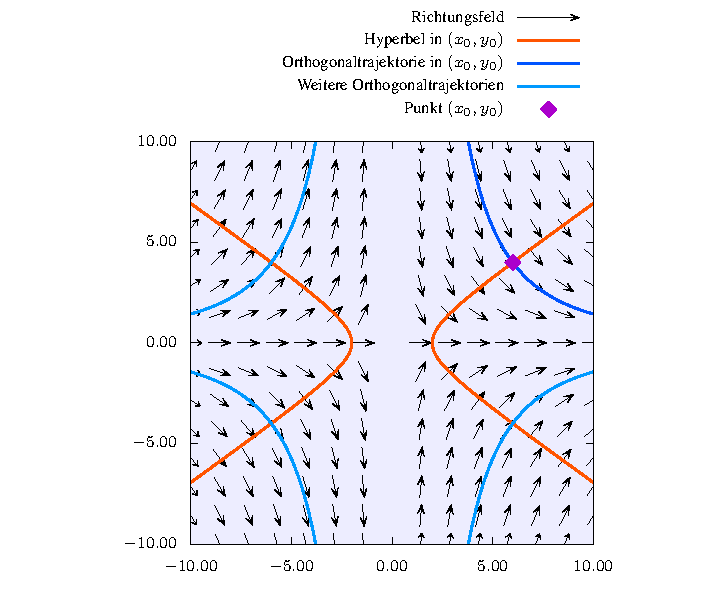
\includegraphics[width=0.95\textwidth]{task-orthogonaltrajektorien_und_richtungsfeld-diagram.pdf}
			\caption{Das Diagramm zeigt das Richtungsfeld der Orthogonaltrajektorien und das Beispiel einer zugehörigen Hyperbel.}
		\end{figure}
	\end{atiSubtaskSolutions}
\end{atiSolution}